
%Results body
%Created SS 04-14

\section{Results}\label{results}

\subsection{Observing Optical Pumping and rf Coupling}\label{ObservingOpticalPumpingandrfCoupling}

With the external magnetic field applied, laser light is used to optically pump rubidium atoms into a preferential spin state.  To observe this pumping, we measure the transmission of laser light through the cell using a photodetector.  Transmission will increase when atoms are optically pumped into an excited $m_F$ state and no longer absorb the laser light. This sample data is observed on an oscilloscope as shown in Fig. \ref{fig:raw_data}.  We observe roughly a $10\%$ increase in transmission due to the optical pumping of the $3\rightarrow3$ transition for $^{85}$Rb.
\begin{figure}[htbp]
\begin{center}
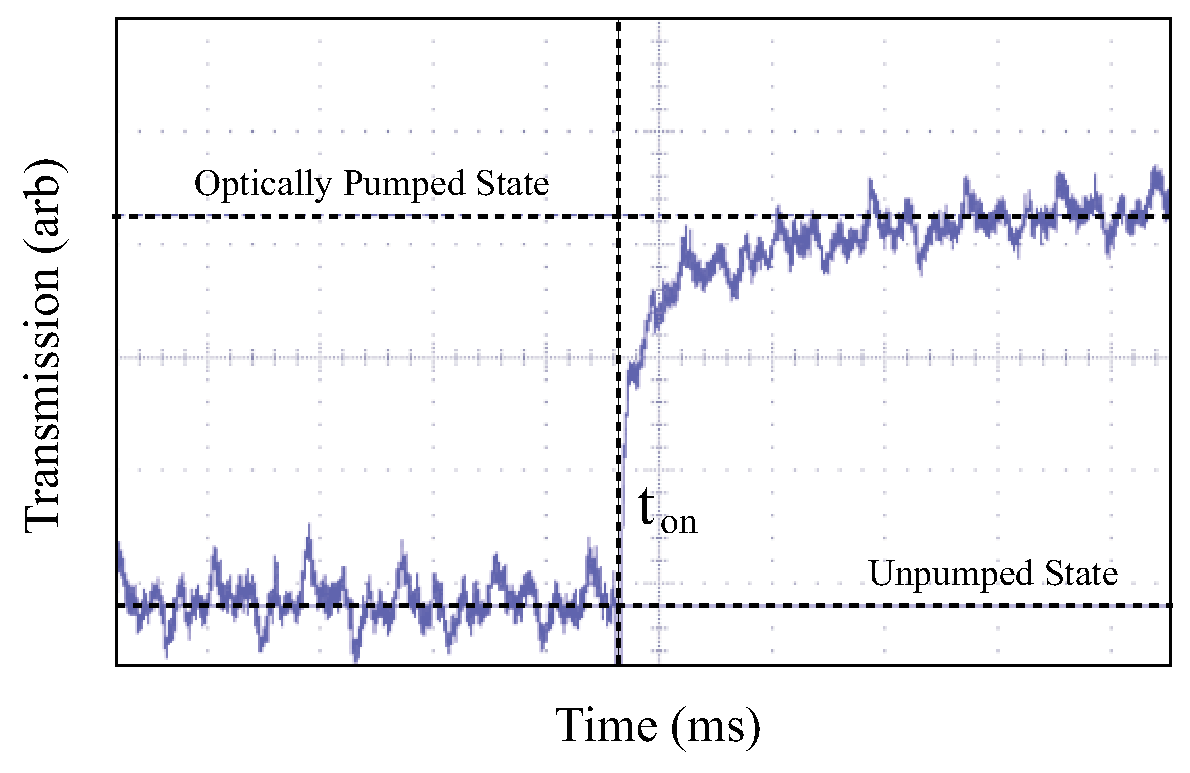
\includegraphics[height=70mm]{./figures/raw_data.eps}
\caption{\small{Sample oscilloscope data of optical pumping. At $t=t_{on}$, the external magnetic field is turned on. The subsequent Zeeman splitting enables the rubidium atoms to be optically pumped to preferential $m_F$ state using laser light.  Optical pumping is observed in the increase of transmission to a higher steady state level.}}
\label{fig:raw_data}
\end{center}
\end{figure}

A radiofrequency magnetic field is used to disrupt the optically pumped steady state by coupling the pumped $m_F$ state to the next (lower) $m_F$ state.  This coupling creates a transient phenomenon which is characterized by the decrease in signal from the pumped level to some new steady state.  In order to closely analyze the transient portion due rf interference, a chopped rf signal is used.  
\begin{figure}[htbp]
\begin{center}
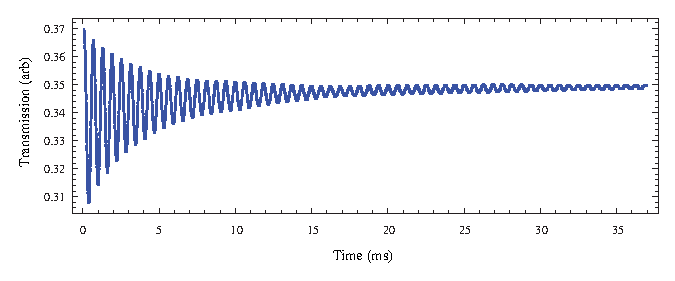
\includegraphics[height=70mm]{./figures/rabi.eps}
\caption{\small{Rabi oscillations resulting from radiofrequency coupling of $m_F$ states while optically pumping $^{85}$Rb.}}
\label{fig:rabi}
\end{center}
\end{figure}
The depumping caused by the $m_F$ coupling combined with optical pumping creates Rabi oscillations in the transient portion between the fully state and the new equilibrium.  This phenomenon is shown in Fig. \ref{fig:rabi}.  The oscillations signify periodic fluctuations in spin state populations due to the $m_F$ coupling, as predicted by Eqn.~\ref{eqn:rabi}.

\subsection{Measuring Linewidth and Optical Pumping Resonance}\label{MeasuringLinewidthandOpticalPumpingResonance}

Using a lock-in amplifier, we measure the amplitude of Rabi oscillations as a function of the applied radiofrequency.  We use a LabView program in order to select and step through a range of radiofrequencies in order to observe the Lorentzian resonance.  This data was taken for both $^{85}$Rb and $^{87}$Rb. This data is shown in Fig. \ref{fig:rawcurve}.    
\begin{figure}[h!]
\begin{center}
\subfigure[$^{85}$Rb ($3\rightarrow3$)]{\label{fig:edge-a}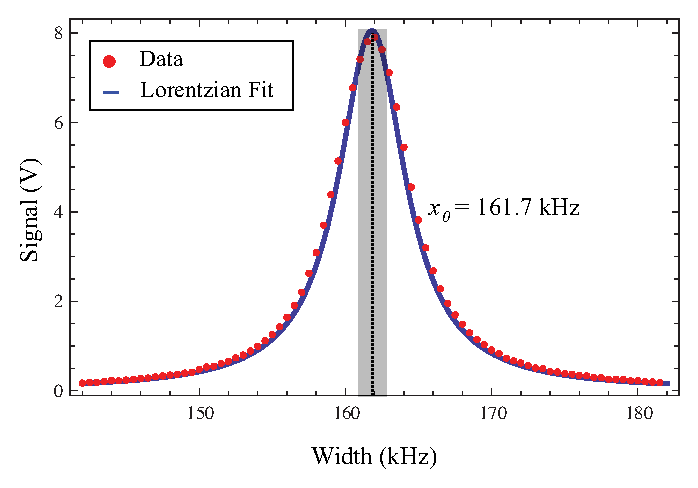
\includegraphics[height=50mm]{./figures/85raw_width.eps}}
\hspace{-1mm}
\vspace{-2mm}
\subfigure[$^{87}$Rb ($2\rightarrow2$)]{\label{fig:edge-b}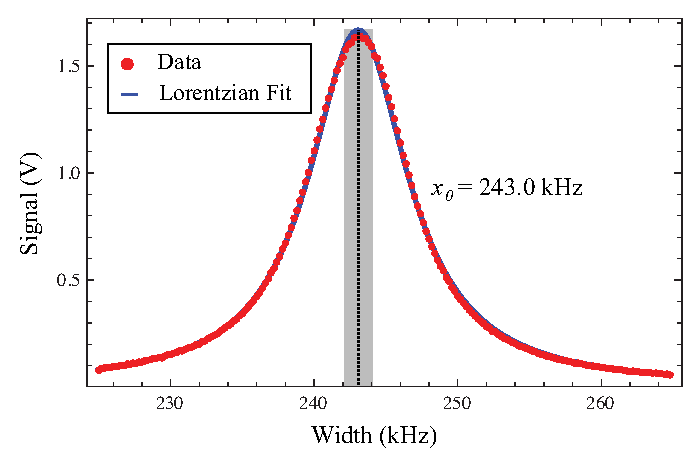
\includegraphics[height=50mm]{./figures/87raw_width.eps}}
\vspace{-2mm}
\caption{\small{Optical pumping resonances for rubidium isotopes. Fitting this data to Lorentzian distributions, we are able to determine the resonant frequencies at which $m_F$ states couple. For $^{85}$Rb and $^{87}$Rb, these resonant frequencies are $161.0 \pm 0.8$ kHz and $243.1\pm 0.3$ kHz respectively. We are also able to use this data to measures the linewidth.}}
\label{fig:rawcurve}
\end{center}
\end{figure}
This data was fit to Lorentzian distributions. These fits were then used to calculate the resonant frequencies.  The resonant $m_F$ coupling frequencies for $^{85}$Rb and $^{87}$Rb are $161.0 \pm 0.8$ kHz and $243.1\pm 0.3$ kHz respectively.  

Further measurements are taken using the $^{85}$Rb $3\rightarrow3$ transition to determine the effect of radiofrequency amplitude and laser light intensity on the linewidth of the resonance. By independently varying either of these variables, several resonances are measured.  Using a \emph{Mathematica} program, the linewidths of these resonances are calculated and plotted with respect to both radiofrequency amplitude and laser light intensity.  This data is shown in Fig. \ref{fig:linewidths}.
\begin{figure}[h!]
\begin{center}
\subfigure[Varying rf Amplitude]{\label{fig:edge-a}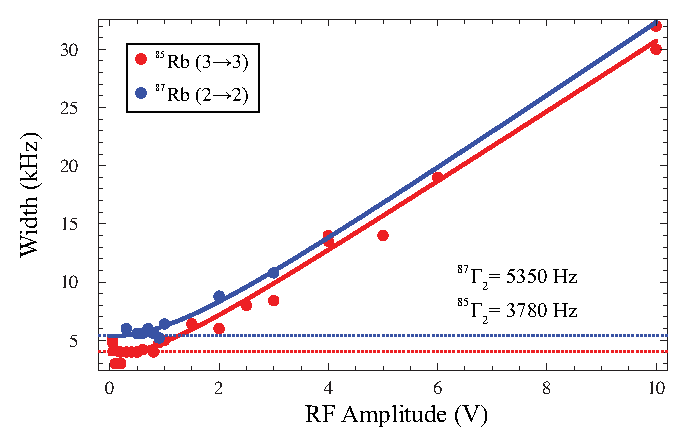
\includegraphics[height=50mm]{./figures/amp_width.eps}}
\hspace{-1mm}
\vspace{-2mm}
\subfigure[Varying Intensity]{\label{fig:edge-b}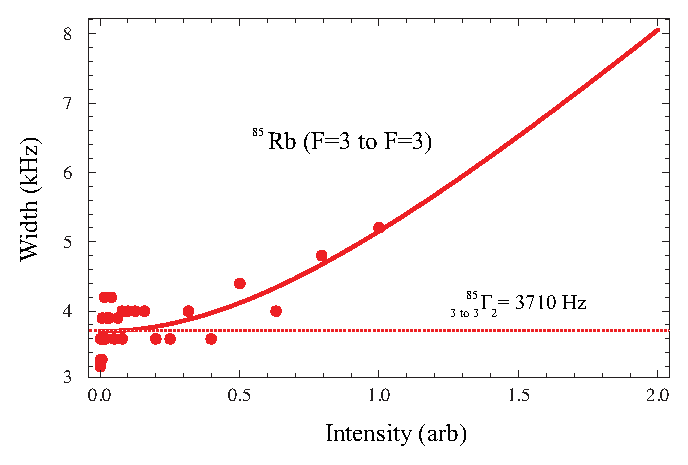
\includegraphics[height=50mm]{./figures/intensity_width.eps}}
\vspace{-2mm}
\caption{\small{Power broadening of rubidium linewidths due to laser light intensity and rf amplitude.  The data in (a) is fit to $\alpha \sqrt{1+\beta x^2}$ whereas the the data in (b) is fit to $\alpha \sqrt{1+\beta x}$.  With these fits we are able to determine the natural $\gamma_2$ linewidths for $^{85}$Rb and $^{87}$Rb which are found to be $3.70 \pm 0.48$ kHz and $5.35 \pm 0.47$ kHz respectively.  Error is either identified by the thickness of the points (a) or error bars (b).}}\label{fig:linewidths}
\end{center}
\end{figure}
The variable being held constant was chosen in a regime in which it would not have a confounding effect on the linewidth--\emph{i.e.} while varying light intensity, radiofrequency amplitude was minimized and \emph{vice versa}.  We expect the $\gamma_2$ linewidth to be given by 
Eqns. \ref{eq:rfbroad} and \ref{eq:lightbroad}. Accordingly, the data for varying rf amplitude is fit to a $\alpha \sqrt{1+\beta x^2}$ model whereas the data for varying light intensity is fit to a $\alpha \sqrt{1+\beta x}$ model.  Both fits are done using nonlinear regression analysis (See Appendix \ref{nonlinearregressionanalysis}).  Our data shows very good agreement with the theoretical prediction for power broadening due to laser light intensity and applied rf field.

We would expect the natural linewidths for each measurement process to be the same, since we assume there is only one power-broadening factor in each set of measurements. From our fitting analysis we find the natural $\gamma_2$ linewidths to be $3.78 \pm 0.46$ kHz and $3.63 \pm 0.14$ kHz for varying radiofrequency amplitude and light intensity respectively.  Given the error for this measurement, the two values are in good agreement. From here on we take the natural $\gamma_2$ linewidth for $^{85}$Rb to be $3.70 \pm 0.48$ kHz. The natural  $\gamma_2$ linewidth for $^{87}$Rb was also measured by varying radiofrequency amplitude and calculated to be $5.35 \pm 0.47$ kHz.

\subsection{Measuring $T_1$ Relaxation and Optical Pumping Time}\label{MeasuringT1RelaxationandOpticalPumpingTime}

Using an optical chopper as described in Section \ref{measurementoft1}, we observe transient optical pumping without rf interference and without turning off the external magnetic field.  In doing so we can indirectly observe $T_1$ relaxation of $^{85}$Rb for the $3 \rightarrow 3$ transition.  For this indirect measurement we observe the decrease in the fluorescence signal over a certain amount of time during which the laser light is blocked.  By measuring the relative decrease in signal height for different dark times, we can determine the $T_1$ relaxation time. When unblocked, the laser light again begins to optically pump the atoms.  Sample data of this procedure is shown in Fig. \ref{fig:chop}.
\begin{figure}[htbp]
\begin{center}
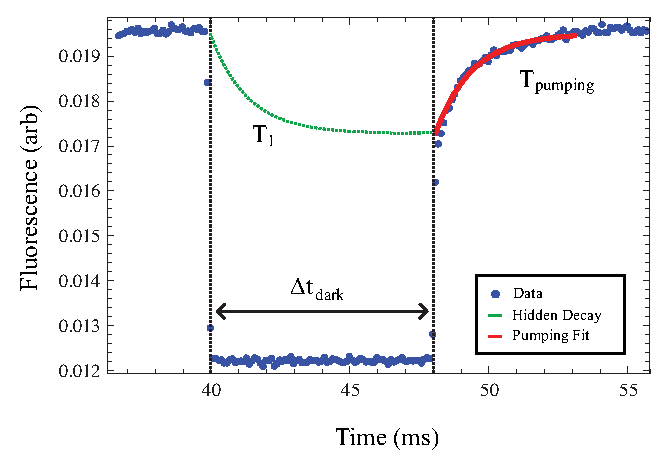
\includegraphics[height=70mm]{./figures/raw_chop.eps}
\caption{\small{Sample data for the $T_1$ and optical pumping time measurement.  An optical chopper blocks the laser lights for some duration $\Delta t$, called the dark time.  During this dark time, the number of atoms in the excited $m_F$ state decreases due to $T_1$ relaxation.  Because the laser is blocked, this decay can only be indirectly measured.  After the dark time, laser light is able to pass through the chopper and optically pump the rubidium atoms.  The red fit is used to determine both the optical pumping time constant and the relative decrease in signal during the dark time. The hidden decay is shown purely for explanatory reasons and is not a fit to the data.}}
\label{fig:chop}
\end{center}
\end{figure}
By setting the optical chopper to different frequencies, we can measure measure the relative decrease in signal for different dark times and thus construct the hidden exponential decay derived in Section \ref{rateequations}.  Moreover, by fitting the subsequent rise in signal following the unblocking of laser light, we can calculate the optical pumping time constant by fitting to an exponential rise.  Further calculation and analysis of this data is done in Section \ref{DeterminationofTimes}.

\subsection{Measuring Spin Exchange Between $^{85}$Rb and $^{87}$Rb}\label{MeasuringSpinExchange}
By optically pumping $^{85}$Rb and coupling the $m_F$ states of $^{87}$Rb we observe spin exchange between the isotopes. To measure the spin exchange process, we use the lock-in amplifier to measure the amplitude of the Rabi oscillations of $^{85}$Rb atoms which have been excited by the Rabi oscillations of the $^{87}$Rb atoms.  This data is similar to the Lorentzian resonances shown in Fig. \ref{fig:rawcurve}.  This process is repeated while pumping $^{85}$Rb atoms and observing the spin exchange resulting in subsequent Rabi oscilliation of $^{87}$Rb atoms.

In order to determine the natural linewidth of both spin exchange processes we measure the linewidths while varying rf amplitude (this procedure is identical to the one used in Section \ref{MeasuringLinewidthandOpticalPumpingResonance}).  This data is fit to $\alpha \sqrt{1+\beta x^2}$ again using nonlinear regression analysis (shown in Fig. \ref{fig: spinexchange}).
\begin{figure}[htbp]
\begin{center}
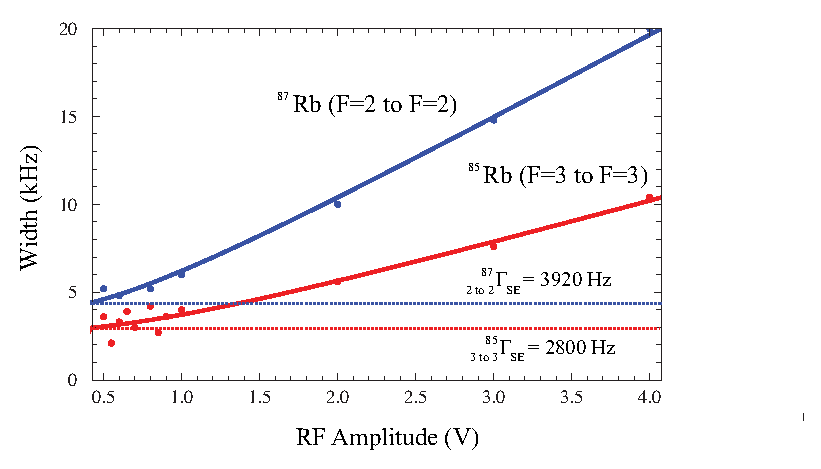
\includegraphics[height=70mm]{./figures/spin_exchange.eps}
\caption{\small{Power broadening of the rubidium spin exchange linewidths due to rf amplitude. By fitting to $\alpha \sqrt{1+\beta x^2}$, we are able to determine the natural spin exchange line widths for $^{85}$Rb and $^{87}$Rb which are found to be $2.80 \pm 0.28$ and kHz $3.92 \pm 0.71$ kHz respectively.  Error is identified by the thickness of the points.}}\label{fig: spinexchange}
\end{center}
\end{figure}
We find the natural linewidths for the spin exchange processes to be $2.80 \pm 0.28$ kHz and $3.92 \pm 0.71$ kHz for $^{85}$Rb and $^{87}$Rb respectively.